\documentclass[margin=0px]{article}

\usepackage{listings}
\usepackage[utf8]{inputenc}
\usepackage{graphicx}
\usepackage{float}
\usepackage[a4paper, margin=1in]{geometry}
\usepackage{amsthm}
\usepackage{amssymb}

\newenvironment{tetel}[1]{\paragraph{#1 \\}}{}
% A dokument itt kezdődik

\title{Záróvizsga tételsor \\ \large 18. Adatbázisok tervezése és lekérdezése}
\date{}
\author{Fekete Dóra}

\begin{document}

	\maketitle
	
	\begin{tetel}{Adatbázisok tervezése és lekérdezése}
			Relációs adatmodell, egyed-kapcsolat modell és átalakítása relációs adatmodellbe. Relációs algebra, SQL. Az SQL procedurális kiterjesztése (PL/SQL vagy PSM). Relációs adatbázis-sémák tervezése, normálformák, dekompozíciók.
	\end{tetel}
	
	\section{Relációs adatmodell, egyed-kapcsolat modell és átalakítása relációs adatmodellbe}
	
	\subsection{Relációs adatmodell}
	
	\textit{Relációs adatmodell}: adatok gyűjteményét kezeli. \\
	\textit{Reláció}: a gyűjtemény megadása (tábla). \\
	\textit{Adatmodell}: a valóság fogalmainak, kapcsolatainak, tevékenységeinek magasabb szintű ábrázolása, számítógép és felhasználó számára is megadja, hogy hogyan néznek ki az adatok. Adatok leírására szolgáló jelölés. \\
	\textit{Részei}:
	\begin{enumerate}
		\item az adat struktúrája
		\item az adaton végezhető műveletek
		\item az adatokra tett megszorítások
	\end{enumerate}
	
	Egyéb fogalmak:
	\begin{itemize}
		\item Relációséma: \textit{relációnév(sortípus)}, $R(A_1,...A_n)$
		\item Előfordulás: példány, a sortípusnak megfelelő \textit{véges sok} sor, $\{t_1,...t_m\}$, ahol $t_i = <v_i1...v_in>$
		\item Attribútumok: adattípus : sortípus, $<$attr.név$_1$ : értéktípus$_1$,...$>$
		\item Kulcsok: Egyszerű kulcs 1 attribútumból áll, összetett többől, nem lehet a relációban két különböző sor, aminek azonos a kulcsa.
		\item Külső kulcs: Idegen kulcs. $R(A_1,...A_m)$ reláció, $X=\{A_{i_1},...A_{i_k}\}$ kulcs. $S(B_1,...B_n)$ reláció, $Y=\{B_{j_1},...B_{j_k}\}$ idegen kulcs, ami az $X$-re hivatkozik a megadott attribútum sorrendben: $B_{j_1}$ az $A_{i_1}$-re stb.
		\item Hivatkozási épség: megszorítás a két tábla együttes előfordulására. Ha $s \in S$ sor, akkor $\exists t \in R$ sor: $s[B_{j_1},...B_{j_k}] = t[A_{i_1},...A_{i_k}]$.
	\end{itemize}
	A relációs adatmodell több szempontból is előnyös, amik miatt elterjedt és kifinomult. Az adatmodell egy egyszerű és könnyen megérthető strukturális részt tartalmaz. A természetes táblázatos formát nem kell magyarázni, és jobban alkalmazható. A relációs modellben a fogalmi-logikai-fizikai szint teljesen szétválik, nagyfokú logikai és fizikai adatfüggetlenség. A felhasználó magas szinten, hozzá közel álló fogalmakkal dolgozik (implementáció rejtve). Elméleti megalapozottság, több absztrakt kezelő nyelv létezik, például relációs algebra (ezen alapul az SQL automatikus és hatékony lekérdezés optimalizálása). Műveleti része egyszerű kezelői felület, szabvány SQL. \\ \\ 
	
	\textit{Relációs adatbázis felépítése}: Az adatbázis tulajdonképpen relációk halmaza. A megfelelő relációsémák halmaza adja az adatbázissémát (jelölése dupla szárú $\mathbb{R}$), $\mathbb{R} = \{R_1 , ... , R_k\}$. A hozzá tartozó előfordulások az adatbázis-előfordulás. Előfordulás tartalma: egyes relációk előfordulásai. Ez a koncepcionális szint, vagyis a fogalmi modell. Fizikai modell: a táblát valamilyen állományszerkezetben jeleníti meg (például szeriális állományban). A relációs adatbázis-kezelők indexelnek, indexelési mód: pl. B+ fa.
	
	\subsection{Egyed-kapcsolat modell}
	
	Elemei:
	\begin{itemize}
		\item Egyedhalmazok: hasonló egyedek összessége
		\item Attribútumok: megfigyelhető tulajdonságok, megfigyelt értékek, egyedek tulajdonságai
		\item Kapcsolatok: más egyedhalmazokkal való kapcsolatok
		\item Séma: $E(A_1,...A_n)$ egyedhalmaz séma, $E$ név, $A_i$ tulajdonság, $DOM(A_i)$ a lehetséges értékek halmaza, pl \textit{tanár(név, tanszék)}
		\item Előfordulás: Konkrét egyedek (entitások), $E=\{e_1,...e_m\}, e_i(k) \in DOM(A_k)$ az egyedek halmaza. Minden attribútumban nem egyezhetnek meg $\to$ (vagyis az összes tulajdonság szuperkulcsot alkot), minimális szuperkulcs = kulcs.
		\item $K(E_1,E_2)$ bináris kapcsolat, $K(E_1,...E_p)$ a kapcsolat sémája. $K$ a kapcsolat neve, $E_i$ az egyedhalmazok sémái, többágú kapcsolat, ha p>2. pl \textit{tanít(tanár, tárgy)}. Többágú kapcsolat átírható megfelelő számú binér kapcsolatra, 3-ágú 3-ra stb.
		\item $K(E_1,...E_p)$ sémájú kapcsolat előfordulása, $K=\{(e_1,...e_p)\}$ egyed p-esek halmaza, ahol $e_i \in E_i$. A kapcsolat előfordulásaira tett megszorítások határozzák meg a kapcsolat típusát.
	\end{itemize}
	Diagram: egyedhalmazok, kapcsolatok típusok, egyenek ábrázolása. \\
	Szerepek: egyedhalmaz önmagával kapcsolódik \\
	Kapcsolat attribútum: két egyedhalmaz együttes függvénye, de egyiké sem külön \\
	Egyedhalmaz: az elsődleges kulcshoz tartozó tulajdonságokat aláhúzzuk \\
	
	\begin{figure}[H]
		\centering
		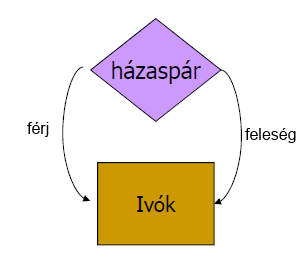
\includegraphics[width=0.3\textwidth]{img/ek4.png}
		\caption{Szerepek}
	\end{figure}
	
	Kapcsolatok típusai (vegyünk hozzá egy $K(E_1,E_2)$ bináris kapcsolatot alapul):
	\begin{itemize}
		\item sok-egy: $K$ előfordulásaiban minden $E_1$-beli egyedhez legfeljebb 1 $E_2$-beli tartozhat, pl \textit{született(név,ország)}
		\item sok-sok: nincs megszorítása, minden $E_1$-beli egyedhez több $E_2$-beli egyed tartozhat, és fordítva, minden $E_2$-beli egyedhez több $E_1$-beli egyed tartozhat, pl \textit{tanul(diák,nyelv)}
		\item egy-egy: sok-egy és egy-sok, vagyis minden $E_1$-beli egyedhez legfeljebb egy $E_2$-beli egyed tartozhat, és fordítva, minden $E_2$-beli egyedhez legfeljebb egy $E_1$-beli egyed tartozhat, pl \textit{házaspár(férfi,nő)}
	\end{itemize}
	Lehet több kapcsolat is két egyedhalmaz között. \\
	\textit{Alosztály}: ,,isa" = ,,az-egy", öröklődés, speciális egy-egy kapcsolat. Összes $E_1$-belihez van egy $E_2$-beli, pl \textit{isa(főnök, dolgozó)}
	\begin{figure}[H]
		\centering
		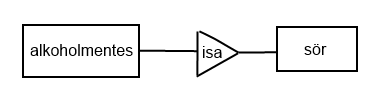
\includegraphics[width=0.6\textwidth]{img/ek2.png}
		\caption{Alosztály}
	\end{figure}
	\textit{Kulcs}: aláhúzással jelölik, összetett kulcsnál több attribútum van aláhúzva \\
	\textit{Szuperkulcs}: Az egyedhalmaz szuperkulcsa egy azonosító, vagyis olyan tulajdonság-halmaz, amelyről feltehető, hogy az egyedhalmaz előfordulásaiban nem szerepel két különböző	egyed, amelyek ezeken a tulajdonságokon megegyeznek. Az összes tulajdonság mindig szuperkulcs.\\
	\textit{Hivatkozási épség}: kerek végződéssel jelölik, megszorítás
	\begin{figure}[H]
		\centering
		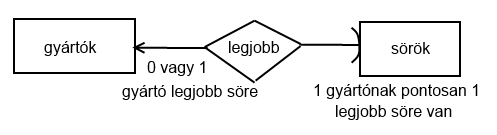
\includegraphics[width=0.6\textwidth]{img/ek3.png}
		\caption{Hivatkozási épség}
	\end{figure}
	\textit{Gyenge egyedhalmaz}: Téglalap dupla kontúrral. Önmagában nem azonosítható egyértelműen.
	\begin{figure}[H]
		\centering
		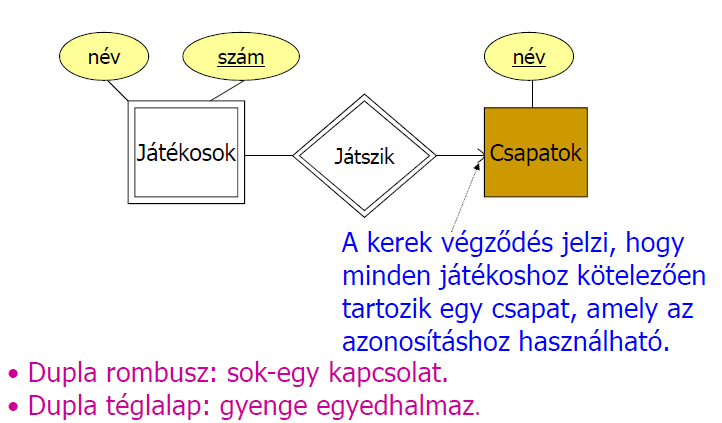
\includegraphics[width=0.45\textwidth]{img/ek5.png}
		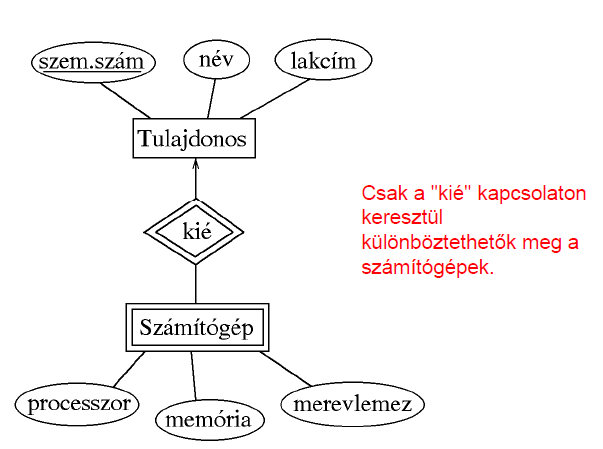
\includegraphics[width=0.45\textwidth]{img/ek6.png}
		\caption{Gyenge egyedhalmaz}
	\end{figure}
	Tervezési alapelvek:
	\begin{itemize}
		\item valósághű modellezés: megfelelő tulajdonságok tartozzanak az egyedosztályokhoz, például a tanár neve ne a diák tulajdonságai közé tartozzon
		\item redundancia elkerülése: az \textit{index(etr-kód,lakcím,tárgy,dátum,jegy)} rossz séma,
		mert a lakcím annyiszor ismétlődik, ahány vizsgajegye van a diáknak, helyette 2 sémát érdemes felvenni: \textit{hallgató(etr-kód,lakcím)}, \textit{vizsga(etr-kód,tárgy,dátum,jegy)}.
		\item egyszerűség: fölöslegesen ne vegyünk fel egyedosztályokat, például a \textit{naptár(év,hónap,nap)} helyett a megfelelő helyen inkább dátum tulajdonságot használjunk
		\item tulajdonság vagy egyedosztály: például a vizsgajegy osztály helyett jegy tulajdonságot
		használjunk.
	\end{itemize}
	
	\subsection{Egyed-kapcsolat modell átalakítása relációs adatmodellbe}
	
	\begin{figure}[H]
		\centering
		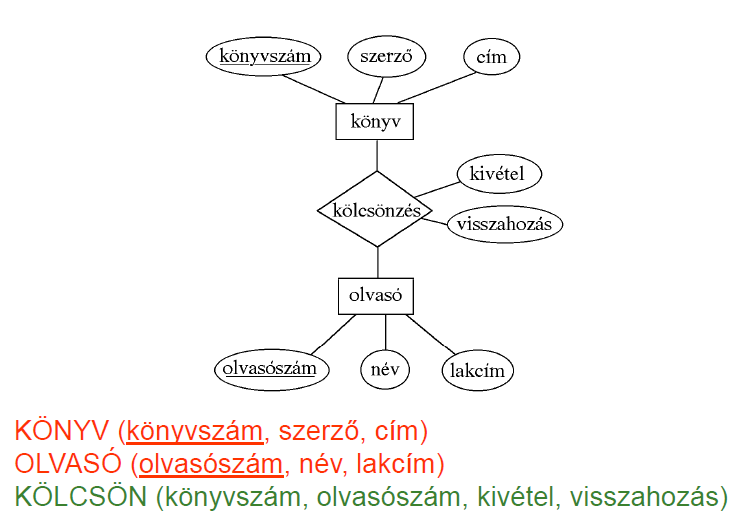
\includegraphics[width=0.6\textwidth]{img/ek7.png}
		\caption{Példa: könyvtár adatmodellje}
	\end{figure}
	\textit{Összetett attribútumok leképezése}: például ha a lakcímet (helység, utca, házszám) struktúrában akarjuk kezelni, akkor fel kell venni a sémába mindet attribútumként.
	\textit{Többértékű attribútumok leképezése}:
	\begin{itemize}
		\item Megadás egyértékűként. Példa: többszerzős könyvnél egy mezőben soroljuk fel az összeset. Nem túl jó, mert nem lehet a szerzőket külön kezelni, és esetleg nem is fér el mind a mezőben.
		\item Megadás többértékűként.
		\begin{itemize}
			\item Sorok többszörözése. Könyves példánál maradva, felveszünk annyi sort, ahány szerző van. Ez redundanciához vezet.
			\item Új tábla felvétele. A \textit{könyv(könyvszám, szerző, cím)} sémát az alábbi két sémával helyettesítjük: \textit{könyv(\underline{könyvszám}, cím)}, \textit{szerző(\underline{könyvszám}, \underline{szerző})}
			\item Sorszámozás. Ha nem mindegy a szerzők sorrendje, akkor az előző megoldásban (új tábla) ki kell egészíteni a szerző táblát egy sorszám mezővel.
		\end{itemize}
	\end{itemize}
	\textit{Kapcsolatok leképezése}:
	\begin{itemize}
		\item egy-egy: beolvasztás az azonos kulcsú sémába. Pl egy könyvet lehet kölcsönözni: KÖLCSÖN(\underline{könyvszám}, olvasószám, \textbf{kivétel}) kapcsolatsémából KÖNYV (\underline{könyvszám}, szerző, cím, olvasószám, \textbf{kivétel}), OLVASÓ (\underline{olvasószám}, név, lakcím) lesz. Itt a kapcsolatsémában az olvasószám is kulcs, és felvehetnénk úgy is, hogy az legyen a kulcs. Ez esetben az OLVASÓ-ba kell beolvasztani.
		\item sok-egy: beolvasztás a ,,sok"-ba. Tehát a példát követve, ha több könyvet lehet kölcsönözni, akkor a könyvszámnak kell a kulcsnak lennie, és csak a KÖNYV-be olvaszthatjuk be.
		\item sok-sok: új tábla. Ha a korábbi kölcsönzések is el vannak tárolva, akkor a kulcsban benne van vagy a kivétel, vagy a visszahozás. Ekkor egyik táblába sem lehet beolvasztani, új táblát kell létrehozni. A séma ez lehet: KÖNYV (\underline{könyvszám}, szerző, cím), OLVASÓ (\underline{olvasószám}, név, lakcím), KÖLCSÖN (\underline{könyvszám}, olvasószám, \underline{kivétel}, visszahozás).
	\end{itemize}
	
	\textit{Átalakítás} E/K modell $\to$ relációs adatmodell:
	\begin{itemize}
		\item egyedhalmaz séma $\to$ relációséma
		\item tulajdonságok $\to$ attribútumok
		\item (szuper)kulcs $\to$ (szuper)kulcs
		\item egyedhalmaz előfordulása $\to$ reláció
		\item egyed $\to$ $e(A_1)...e(A_n)$ sor
		\item $R(E_1,...E_p, A_1,...A_q)$ kapcsolati séma ($E_i$ egyedhalmaz, $A_j$ tulajdonság) $\to$ $R(K_1,...K_p, A_1,...A_q)$ relációséma ($K_i$ az $E_i$ (szuper)kulcsa)
	\end{itemize}
	Átnevezhetjük, hogy ne legyen kétszer ugyanaz. \\
	isa esetén a speciális osztályhoz hozzávesszük az általános osztály (szuper)kulcsát. Gyenge entitáshoz a meghatározó kapcsolatok kulcsait vesszük hozzá. \\
	\textit{Összevonás} akkor lehet, ha az egyikben idegenkulcs van a másikra. Illetve akkor, ha sok-egy kapcsolatnak felel meg az egyik reláció, a másik pedig a sok oldalon álló egyedhalmaz reláció. Pl Ivók(név, cím) és Kedvenc(ivó,sör) összevonható, és kapjuk az Ivó1(név,cím,kedvencSöre) sémát. \\
	\begin{figure}[H]
		\centering
		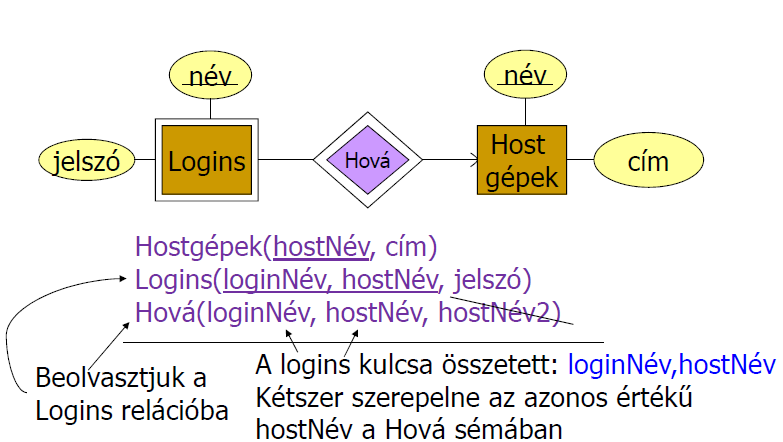
\includegraphics[width=0.6\textwidth]{img/ek8.png}
		\caption{Gyenge egyedhalmaz átírása}
	\end{figure}
	\begin{figure}[H]
		\centering
		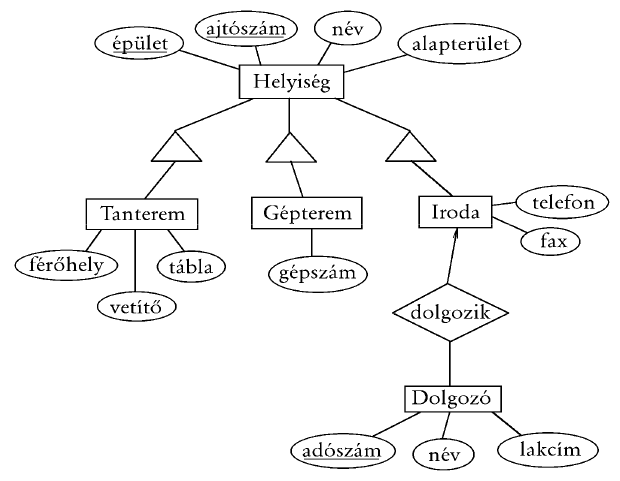
\includegraphics[width=0.6\textwidth]{img/ek9.png}
		\caption{Példa alosztály átírására relációkká}
	\end{figure}
	\textit{Alosztály átírása}:
	\begin{itemize}
		\item Egyed-kapcsolatos: modellben legyen 1 reláció minden alosztályra, de az általánosból csak a kulcsokat vesszük hozzá a saját attribútumokhoz.\\
		Minden altípushoz külön tábla, egy egyed több táblában is szerepelhet. Főtípus táblájában minden egyed szerepel, plusz annyi altípuséban, amennyiben szerepel. Hátrány: több táblában keresés.
		\begin{figure}[H]
			\centering
			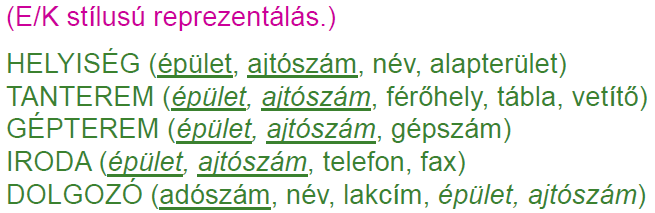
\includegraphics[width=0.6\textwidth]{img/ek.png}
			\caption{E/K stílusú}
		\end{figure}
		\item Nullértékes: 1 reláció van összesen, ha nincs a speciális tulajdonság, akkor NULL-t írunk a helyére.\\
		Attribútumok uniója szerepel a táblában. Hátrány, hogy sok NULL van a táblában, típusinformációt is elveszíthetünk (például ha a gépteremnél a gépszám nem ismert, és ezért NULL, akkor a gépterem lényegében az egyéb helyiségek kategóriájába kerül). 
		\begin{figure}[H]
			\centering
			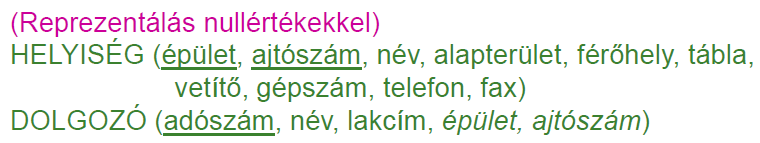
\includegraphics[width=0.6\textwidth]{img/null.png}
			\caption{NULL értékes}
		\end{figure}
		\item Objektumorientált: 1 reláció minden alosztályra, összes tulajdonság felsorolva az örököltből is. \\
		Minden altípushoz külön tábla, egy egyed csak 1 táblában szerepel. Hátrányok: kombinált altípushoz új altípus felvétele szükséges, keresés gyakran több táblán keresztül.
		\begin{figure}[H]
			\centering
			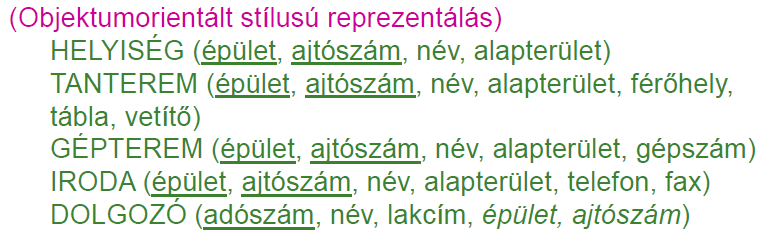
\includegraphics[width=0.6\textwidth]{img/oo.png}
			\caption{Objektumorientált}
		\end{figure}
	\end{itemize}
	
	\section{Relációs algebra, SQL}
	
	\subsection{Relációs algebra}
	
	Algebra műveleteket és atomi operandusokat tartalmaz. \\
	\textit{Relációs algebra}: az atomi operandusokon és az algebrai kifejezéseken végzett műveletek alkalmazásával kapott relációkon műveleteket adunk meg, kifejezéseket építünk (a kifejezés felel meg a kérdés szintaktikai alakjának). Fontos tehát, hogy minden művelet végeredménye reláció, amelyen további műveletek adhatók meg. A relációs algebra atomi operandusai a következők: a relációkhoz tartozó változók; konstansok, amelyek véges relációt fejeznek ki.
	\textit{Műveletek}:
	\begin{itemize}
		\item Halmazműveletek: Reláció előfordulás véges sok sorból álló halmaz. Így értelmezhetők a szokásos halmazműveletek: az unió (az eredmény halmaz, csak egyszer szerepel egy sor), értelmezhető a metszet és a különbség. \\
		R, S azonos típusú, R $\cup$ S és R $-$ S típusa ugyanez \\
		Az alapműveletekhez az unió és különbség tartozik, metszet műveletet származtatjuk: $R \cap S = R - (R - S)$
		\item Vetítés (projekció): Adott relációt vetít le az alsó indexben szereplő attribútumokra (attribútumok számát csökkentik). $\Pi_{lista}(R)$, ahol $\{A_{i_1},...A_{i_k}\}$ R sémájában levő attribútumok egy részhalmazának felsorolása. Reláció soraiból kiválasztja az attribútumoknak megfelelő $A_{i_1},...A_{i_k}$-n előforduló értékeket, ha többször előfordul, akkor a duplikátumokat kiszűrjük (hogy halmazt kapjunk).
		\item Kiválasztás (szűrés): Kiválasztja az argumentumban szereplő reláció azon sorait, amelyek eleget tesznek az alsó indexben szereplő feltételnek. $\sigma_F(R) = \{t|t \in R$ és $t$ kielégíti az $F$ feltételt$\}$ \\
		A feltétel lehet elemi vagy összetett. Elemi: $A_i \Theta A_j$, $A_i \Theta c$, ahol $c$ konstans, $\Theta$ pedig $=, \neq, <, >, \geq, \leq$. Összetett: ha $B_1, B_2$ feltétel, akkor $\not B_1, B_1 \cap B_2, B_1 \cup B_2$ és a zárójelezések is feltétel.
		\item Természetes összekapcsolás: Szorzásjellegű műveletek közül csak ez az alapművelet. Nő az attribútumok száma. A közös attribútumnevekre épül. $R \bowtie S$ azon sorpárokat tartalmazza R-ből illetve S-ből, amelyek R és S azonos attribútumain megegyeznek. $R \bowtie S$ típusa a két attribútumhalmaz uniója.
		\item Átnevezés: Reláció önmagával vett szorzatát ki tudjuk fejezni vele. $\rho_{T(B_1,...B_k)}(R(A_1,...A_k))$, ha az attribútumokat nem akarjuk átnevezni, akkor $\rho_{T}(R)$
	\end{itemize}
	A relációs algebrában a fent felsorolt 6 alapművelet van. Ez egy \textit{minimális készlet}, vagyis bármelyiket elhagyva az a többivel nem fejezhető ki. \\
	Szorzásjellegű műveletnél tekinthetjük a \textit{direkt-szorzatot} alapműveletnek, de a természetes összekapcsolást használják. $R \times S$: az R és S minden sora párban összefűződik, az első tábla minden sorához hozzáfűzzük a második tábla minden sorát. A direkt-szorzat (vagy szorzat, Descartes-szorzat) esetén természetesen nem fontos az attribútumok egyenlősége. A két vagy több reláció azonos nevű attribútumait azonban meg kell különböztetni egymástól (átnevezéssel). \\
	\textit{Monotonitás}: monoton, nem csökkenő kifejezés esetén bővebb relációra alkalmazva az eredmény is bővebb.\\
	A kivonás kivételnek számít az alapműveletek között, mert nem monoton. Következmény ebből, hogy a kivonás nem fejezhető ki a többi alapművelettel. A kivonás nélkül szokás monoton relációs algebrának is nevezni. \\
	\textit{Osztás}: maradékos osztás mintájára. R és S sémája $R(A_1,...,A_n,B_1,...,B_m)$, illetve $S(B_1,...,B_m)$, $Q = R \div S$ sémája $Q(A_1,...,A_n)$. $R \div S$ a legnagyobb (legtöbb sort tartalmazó) reláció, amelyre $( R \div S ) \times S \subseteq R.$ Relációs algebrában: $R(A,B) \div S(B) = \Pi_{A_1,...,A_n}(R) – \Pi_{A_1,...,A_n}( \Pi_{A_1,...,A_n}(R) \times S – R )$\\
	Relációs algebrai kifejezés, mint lekérdező nyelv (L-nyelv). Az alapkifejezések az elemi kifejezések, az összetettek pedig a rajtuk végzett alapműveletek. \\
	\textit{Kifejezés kiértékelése}: összetett kifejezést kívülről befelé haladva átírjuk kiértékelő fává, levelek: elemi kifejezések.
	\begin{figure}[H]
		\centering
		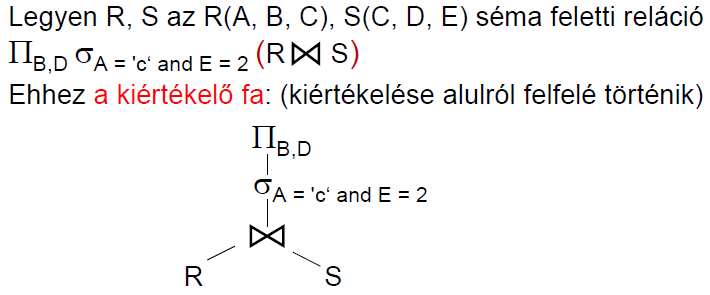
\includegraphics[width=0.6\textwidth]{img/relalg1.png}
		\caption{Kifejezésfa}
	\end{figure}
	
	\subsubsection{Relációs algebra kiterjesztése}
	
	\begin{itemize}
		\item Ismétlődések megszüntetése ($\delta$), select distinct. Multihalmazból halmazt csinál.
		\item Összesítő műveletek és csoportosítás ($\gamma_{lista}$), group by. Összesítő függvények: sum, count, min, max, avg. Itt a $lista$ valamennyi eleme a következők egyike:
		\begin{itemize}
			\item a reláció egy attribútuma: ez az attribútum egyike a csoportosító attribútumoknak (a GROUP BY után jelenik meg).
			\item a reláció egyik attribútumára (ez az összesítési attribútumra) alkalmazott összesítő operátor, ha az összesítés eredményére névvel szeretnénk hivatkozni, akkor nyilat és új nevet használunk.
		\end{itemize}
		R sorait csoportokba osszuk. Egy csoport azokat a sorokat tartalmazza, amelyek a listán szereplő
		csoportosítási attribútumokhoz tartozó értékei megegyeznek, vagyis ezen attribútumok minden egyes különböző értéke egy csoportot alkot. Minden egyes csoporthoz számoljuk ki a lista összesítési attribútumaira vonatkozó összesítéseket. Az eredmény minden egyes csoportra egy sor:
		\begin{enumerate}
			\item a csoportosítási attribútumok és
			\item Az összesítési attribútumra vonatkozó összesítése	(az adott csoport összes sorára)
		\end{enumerate} 
		\item Vetítési művelet kiterjesztése ($\Pi_{lista}$), select kif [as onev]. A $lista$ tartalmazhatja:
		\begin{itemize}
			\item R egy attribútumát,
			\item x $\to$ y, ahol x, y attribútumnevek, s itt x-et y-ra nevezzük át,
			\item E $\to$ y, ahol E R attribútumait, konstansokat, aritmetikai operátorokat és karakterlánc operátorokat tartalmazhat, például: A + 5, C $||$ 'nevű emberek'.
		\end{itemize}
		\item Rendezési művelet ($\tau_{lista}$), order by. $lista = (A_1,...A_n)$ Először $A_1$ attribútum szerint rendezzük R sorait. Majd azokat a sorokat, amelyek értéke megegyezik az $A_1$ attribútumon, $A_2$ szerint, és így tovább. \\
		Ez az egyetlen olyan művelet, amelynek az eredménye se nem halmaz, se nem multihalmaz.
		\item Külső összekapcsolások ($\mathring{\bowtie}$), [left $|$ right $|$ full] outer join. Ez nem relációs algebrai művelet, ugyanis kilép a modellből. $R \bowtie S$ relációt kiegészítjük az R és S soraival, a hiányzó helyekre NULL értéket írva megőrzi a ,,lógó sorokat".
	\end{itemize}
	SQL-ben, és a kiterjesztésben is multihalmazok vannak, vagyis egy sor többször is előfordulhat. \\
	R és S uniójánál n+m előfordulás lesz, metszeténél min[n,m], különbségnél max[0, n-m]. A többi műveletnél nem küszöböljük ki az ismétlődéseket.
	
	\subsection{SQL}
	
	Fő komponensei:
	\begin{itemize}
		\item Adatleíró nyelv, DDL (Data Definition Language): CREATE, ALTER, DROP
		\item Adatkezelő nyelv, DML (Data Manipulation Language): INSERT, UPDATE, DELETE, SELECT \\
		Az SQL elsődlegesen lekérdező nyelv (Query Language): SELECT utasítás (az adatbázisból információhoz jussunk)
		\item Adatvezérlő nyelv, DCL (Data Control Language): GRANT, REVOKE
		\item Tranzakció-kezelés: COMMIT, ROLLBACK, SAVEPOINT
		\item Procedurális kiterjesztések: Oracle PL/SQL (Ada alapján), SQL/PSM (PL/SQL alapján)
	\end{itemize}
	Reláció itt tábla, alapvetően 3-féle: TABLE (alaptábla, permanens), VIEW (nézettábla), WITH utasítással (átmeneti munkatábla).\\
	Séma megadása CREATE utasítással, típus SQL konkrét megvalósítása alapján. Kiegészítő lehetőségek is vannak, pl PRIMARY KEY. Csak egyetlen PRIMARY KEY lehet a relációban, viszont UNIQUE több is lehet, PRIMARY KEY egyik attribútuma sem lehet NULL érték egyik sorban sem. Viszont UNIQUE-nak deklarált attribútum lehet NULL értékű, vagyis a táblának lehet olyan sora, ahol a UNIQUE attribútum értéke NULL, vagyis hiányzó érték. \\ \\
	
	Relációs algebrai kifejezések felírása SELECT-tel:
	\begin{itemize}
		\item SELECT lista FROM táblák szorzata WHERE felt. = $\Pi_{lista}(\sigma_{felt.}$(táblák szorzata))
		\item halmazműveletek: UNION, EXCEPT/MINUS, INTERSECT. Multihalmazból halmaz lesz. ALL kulcsszóval megmarad a multihalmaz.
		\item átnevezés: oszlopnév után szóközzel odaírjuk az új nevet.
	\end{itemize}
	Kiterjesztett műveletek:
	\begin{itemize}
		\item rendezés: ORDER BY, minden más záradék után következik, csökkenő, növekvő sorrend.
		\item ismétlődések megszüntetése: select DISTINCT ...
		\item összesítések (aggregálás): SUM, COUNT, MIN, MAX, AVG a SELECT záradékban. COUNT(*) az eredmény sorainak száma. Ha összesítés is szerepel a lekérdezésben, a SELECT-ben felsorolt attribútumok vagy egy összesítő függvény paramétereként szerepelnek, vagy a GROUP BY attribútumlistájában is megjelennek.
		\item csoportosítás: GROUP BY. 
		\item csoportok szűrése: HAVING. Csoportokat szűr, nem egy-egy sort. Az alkérdésre nincs megszorítás. Viszont az alkérdésen kívül csak olyan attribútumok szerepelhetnek, amelyek: vagy csoportosító attribútumok, vagy összesített attribútomok. (Azaz ugyanazok a szabályok érvényesek, mint a SELECT záradéknál).
	\end{itemize}
	\begin{figure}[H]
		\centering
		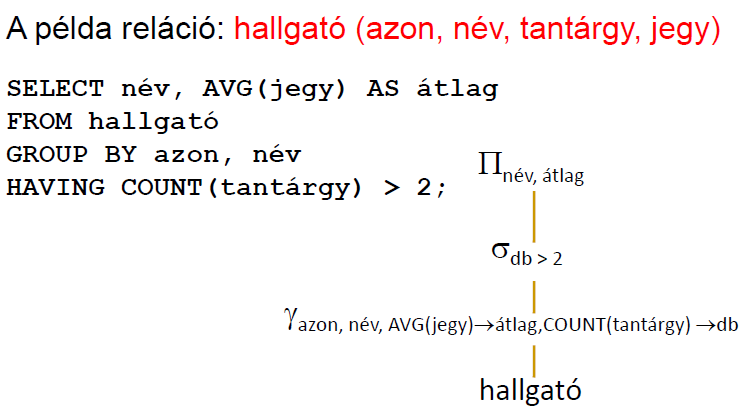
\includegraphics[width=0.6\textwidth]{img/sql2.png}
		\caption{Példa csoportosításra}
	\end{figure}
	WHERE záradéknál SQL-es specialitások:
	\begin{itemize}
		\item Átírható relációs algebrába: BETWEEN ... AND ..., IN(értékhalmaz)
		\item Nem írható át: LIKE karakterláncok összehasonlításánál, IS NULL (ismeretlen vagy nem definiált érték) [emiatt 3-értékű logika SQL-ben: true, false, unknown]
	\end{itemize}
	SELECT utasítás több részből áll, a részeket záradékoknak nevezzük. Három alapvető záradék van:
	\begin{itemize}
		\item SELECT lista (3.) -- milyen típusú sort szeretnénk az eredményben látni? * jelentése: minden attribútum.
		\item FROM Relációnév (1.) -- a tábla neve vagy relációk (táblák) összekapcsolása, illetve szorzata
		\item WHERE feltétel (2.) -- milyen feltételeknek eleget tevő sorokat kiválasztani?
	\end{itemize}
	Több séma összekapcsolása esetén ha egy attribútumnév több sémában is előfordul, akkor kell hozzá a séma is a hivatkozásnál: R.A (R reláció A attribútuma). \\
	\textit{Alkérdéseket} is használhatunk SQL-ben, ezt zárójelbe tevéssel érjük el.\\
	\begin{itemize}
		\item FROM záradékban ilyen módon ideiglenes táblát is létrehozhatunk, ekkor többnyire a sorváltozó nevét is meg kell adni hozzá.
		\item WHERE záradékban az alkérdés eredménye lehet:
		\begin{itemize}
			\item egy skalárérték, vagyis mintha egy konstans lenne
			\item skalár értékekből álló multihalmaz, logikai kifejezésekben használható: EXISTS, [NOT] IN, ANY/ALL (pl x > ANY (alkérdés)).
			\item teljes többdimenziós tábla, használható: EXISTS, [NOT] IN
		\end{itemize}
	\end{itemize}
	Az alkérdés nem korrelált, ha önállóan kiértékelhető, külső kérdés közben nem változik. Korrelált, ha többször kerül kiértékelésre, alkérdésen kívüli sorváltozóból származó értékadással.
	\begin{figure}[H]
		\centering
		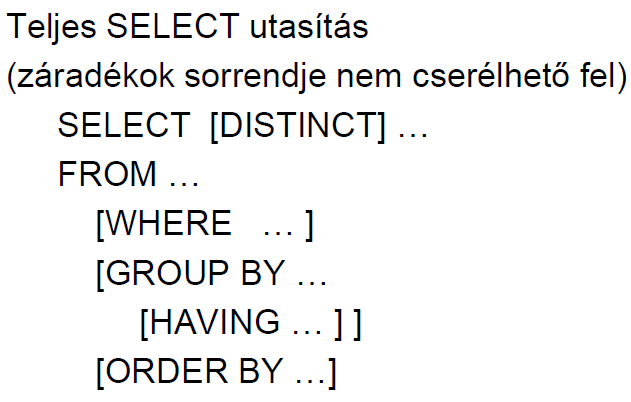
\includegraphics[width=0.45\textwidth]{img/sql1.png}
		\caption{SQL záradékok}
	\end{figure}
	\textit{Összekapcsolások}:
	\begin{itemize}
		\item Descartes-szorzat: R CROSS JOIN S, vagy ,,R,S"
		\item Természetes összekapcsolás: R NATURAL JOIN S
		\item Théta-összekapcsolás: R JOIN S ON <feltétel>
		\item Külső összekapcsolás: R $\{$LEFT $|$ RIGHT $|$ FULL$\}$ OUTER JOIN S. LEFT az R lógó sorait őrzi meg, RIGHT az S-ét, FULL az összeset.
	\end{itemize}
	
	\subsubsection{DML}
	
	A módosító utasítások nem adnak vissza eredményt, mint a lekérdezések, hanem az adatbázis tartalmát változtatják meg. 3-féle módosító utasítás létezik:
	\begin{itemize}
		\item INSERT - sorok beillesztése, beszúrása. Egyetlen sor: INSERT INTO R VALUES ($<$attr. lista$>$). A tábla létrehozásánál ha megadtunk default értékeket attribútumoknál, akkor ha nem adunk meg értéket hozzá, akkor a default lesz, egyébként NULL. Több sor: INSERT INTO R ($<$alkérdés$>$).
		\item DELETE – sorok törlése. DELETE FROM R [WHERE $<$feltétel$>$].
		\item UPDATE – sorok komponensei értékeinek módosítása. UPDATE R SET $<$attribútum értékadások listája$>$ WHERE $<$sorokra vonatkozó feltétel$>$
	\end{itemize}
	\textit{Tranzakciók}: Az adatbázisrendszereket általában több felhasználó és folyamat használja egy időben. Tranzakció = olyan folyamat, ami adatbázis lekérdezéseket, módosításokat tartalmaz. Az utasítások egy ,,értelmes egészt" alkotnak. \\
	ACID: atomicity (vagy az összes vagy egyik utasítás sem hajtódik végre), consistency (konzisztencia, a megszorítások megőrződnek), isolation (elkülönítés, felhasználó számára úgy tűnik, hogy egymás után futnak a tranzakciók), durability (tartósság, befejeződött tranzakció módosításai nem vesznek el). \\
	A COMMIT SQL utasítás végrehajtása után a tranzakció véglegesnek tekinthető. A tranzakció módosításai véglegesítődnek. A ROLLBACK SQL utasítás esetén a tranzakció abortál, azaz az összes utasítás visszagörgetésre kerül. \\
	Többféle elkülönítési szint közül lehet választani, hogy az egy időben történő tranzakciók esetén milyen interakciók engedélyezettek.
	\begin{enumerate}
		\item SERIALIZABLE: ACID tulajdonságok teljesülnek rá. Más tranzakciója közbeni állapotot nem láthat a felhasználó.
		\item REPEATABLE READ: Hasonló a read-commited megszorításhoz. Itt, ha az adatot újra beolvassuk, akkor amit először láttunk, másodszor is látni fogjuk. De második és az azt követő beolvasások után akár több sort is láthatunk.
		\item READ COMMITTED: csak kommitálás utáni adatot láthat, de nem feltétlenül mindig ugyanazt az adatot.
		\item READ UNCOMMITTED
	\end{enumerate}
	
	\subsubsection{DDL}
	
	Adatleíró részt is tartalmaz az SQL.
	\begin{itemize}
		\item CREATE: létrehozás
		\item DROP: eldobja a teljes leírást, és minden, ami ehhez kapcsolódott, elérhetetlen lesz.
		\item ALTER: leírás módosítása
	\end{itemize}
	A \textit{megszorítás} adatelemek közötti kapcsolat, amelyet az AB rendszernek fent kell tartania. Lehet kulcs megszorítás, értékekre, sorokra vonatkozó. Megszorítás módosítása CONSTRAINTS kulcsszóval, önálló megszorítások: CREATE ASSERTION $<$név$>$ CHECK ($<$feltétel$>$). Itt alapvetően az adatbázis bármely módosítása előtt ellenőrizni kell. Egy okos rendszer felismeri, hogy mely változtatások, mely megszorításokat érinthetnek. \\
	Idegen kulcs (R-ről S-re) megszorítást meg kell őrizni, ez kétféleképpen sérülhet: 1. Egy R-be történő beszúrásnál vagy R-ben történő módosításnál S-ben nem szereplő értéket adunk meg. 2. Egy S-beli törlés vagy módosítás ,,lógó" sorokat eredményez R-ben. Védeni többféleképpen lehet: alapértelmezetten nem hajtja végre, továbbgyűrűzésnél igazítjuk a tábla értékeit a változáshoz, set NULL-nál pedig az érintett sorokat NULL-ra állítjuk. \\
	Sor megszorításnál a CREATE utasításon belül a végére tehetünk egy CHECK ($<$feltétel$>$) utasítást. \\ \\
	\textit{Triggerek} olyankor hajtódnak végre, amikor valamilyen megadott esemény történik, mint például sorok beszúrása egy táblába. Az önálló megszorításokkal (assertions) sok mindent le tudunk írni, az ellenőrzésük azonban gondot jelenthet. Az attribútumokra és sorokra vonatkozó megszorítások ellenőrzése egyszerűbb (tudjuk mikor történik), ám ezekkel nem tudunk minden kifejezni. A triggerek esetén a felhasználó mondja meg, hogy egy megszorítás mikor kerüljön ellenőrzésre. A triggereket esetenként ECA szabályoknak (event-condition-action) is nevezik.
	\begin{itemize}
		\item Esemény: általában valamilyen módosítás a adatbázisban, INSERT, DELETE, UPDATE. Mikor?: BEFORE, AFTER, INSTEAD, Mit?: OLD ROW, NEW ROW, FOR EACH ROW, OLD/NEW TABLE, FOR EACH STATEMENT
		\item WHEN feltétel : bármilyen SQL igaz-hamis-(ismeretlen) feltétel.
		\item Tevékenység : SQL utasítás, BEGIN..END, PSM tárolt eljárás
	\end{itemize}
	A triggerek az eddigi megszorításoktól három dologban térnek el:
	\begin{itemize}
		\item A triggereket a rendszer csak akkor ellenőrzi, ha bizonyos események bekövetkeznek. A megengedett események általában egy adott relációra vonatkozó beszúrás, törlés, módosítás, vagy a tranzakció befejeződése.
		\item A kiváltó esemény azonnali megakadályozása helyett a trigger először egy feltételt vizsgál meg.
		\item Ha a trigger feltétele teljesül, akkor a rendszer végrehajtja a triggerhez tartozó tevékenységet. Ez a művelet ezután megakadályozhatja a kiváltó esemény megtörténtét, vagy meg nem történtté teheti azt.
	\end{itemize}
	\textit{Nézettáblák}: A nézettábla olyan reláció, amit tárolt táblák (alaptáblák) és más nézettáblák felhasználásával definiálunk. Kétféle létezik: 1. virtuális = nem tárolódik az adatbázisban; csak a relációt megadó lekérdezés. 2. Materializált = kiszámítódik, majd tárolásra
	kerül. CREATE [MATERIALIZED] VIEW $<$név$>$ AS $<$lekérdezés$>$. A nézettáblák ugyanúgy kérdezhetők le, mint az alaptáblák. A nézettáblákon keresztül az alaptáblák néhány esetben módosíthatóak is, ha a rendszer a módosításokat át tudja vezetni. Virtuális nézetet nem lehet módosítani, mert nem létezik, de egy INSTEAD OF triggerrel mégis végrehajtathatjuk a változtatásokat.

	\section{Az SQL procedurális kiterjesztése (PL/SQL vagy PSM)}
	
	\subsection{PSM}
	
	Amikor az SQL utasításokat egy alkalmazás részeként, programban használjuk, a következő problémák léphetnek fel:
	\begin{itemize}
		\item Osztott változók használata: közös változók a nyelv és az SQL utasítás között (ott használható SQL utasításban, ahol kifejezés használható).
		\item A típuseltérés problémája: Az SQL magját a relációs adatmodell képezi. Tábla – gyűjtemény, sorok multihalmaza, mint adattípus nem fordul elő a magasszintű nyelvekben. A lekérdezés eredménye hogyan használható fel? Három esetet különböztetünk meg attól függően, hogy a SELECT FROM [WHERE stb] lekérdezés eredménye skalárértékkel, egyetlen sorral vagy egy listával (multihalmazzal) tér-e vissza. Utóbbinál kurzor használata, az eredmény soronkénti bejárása. Egyetlen sornál SELECT $e_1,...e_n$ INTO vált$_1$,...vált$_n$
 	\end{itemize}
 	Háromféleképpen is megközelíthetjük programozási szempontból:
 	\begin{enumerate}
 		\item SQL kiterjesztése procedurális eszközökkel, az adatbázis séma részeként tárolt kódrészekkel, tárolt modulokkal (pl. PSM = Persistent Stored Modules, Oracle PL/SQL).
 		\item Beágyazott SQL (sajátos előzetes beágyazás EXEC SQL. - Előfordító alakítja át a befogadó gazdanyelvre/host language, pl. C)
 		\item Hívásszintű felület: hagyományos nyelvben programozunk, függvénykönyvtárat használunk az adatbázishoz való hozzáféréshez (pl. CLI = call-level interface, JDBC, PHP/DB)
 	\end{enumerate}
 	PSM: Persistent Stored Procedures. SQL utasítások és konvencionális elemek (if, while stb) keverékéből áll. Olyan dolgokat is meg lehet csinálni, amit önmagában az SQL-ben nem.
 	\begin{figure}[H]
 		\centering
 		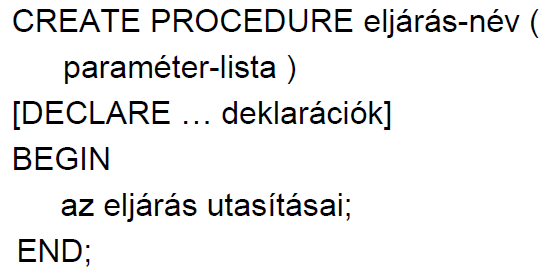
\includegraphics[width=0.45\textwidth]{img/psm1.png}
 		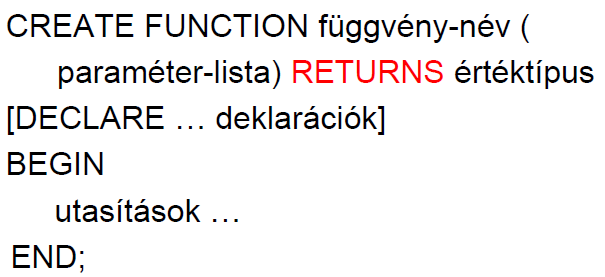
\includegraphics[width=0.45\textwidth]{img/psm2.png}
 		\caption{PSM tárolt eljárás és függvény szerkezete}
 	\end{figure}
 	A tárolt eljárásnak adhatunk paramétereket is, ezek IN, OUT és INOUT módúak lehetnek. Ezek mellé még a paraméter nevét és típusát is meg kell adni, mód-név-típus hármas. Tárolt függvények esetén csak IN módú paramétereink lehetnek. \\
 	Néhány fontosabb utasítás:
 	\begin{itemize}
 		\item Eljárás meghívása a CALL $<$eljárás neve$>$ ($<$argumentumlista$>$) utasítással történik.
 		\item Függvénynél a RETURN utasítás határozza meg a visszatérési érték típusát. Fontos, hogy ezen utasítás hatására nem terminál a függvény.
 		\item Változót deklarálásához ezt használjuk: DECLARE $<$név$>$ $<$típus$>$.
 		\item értékadás: SET $<$változó$>$ = $<$kifejezés$>$.
 		\item BEGIN...END között vannak az utasítások, pontosvesszővel választjuk el őket.
 		\item címke: utasításnak lehet adni, név és kettőspont elé írásával.
 		\item SQL utasítások, DML, MERGE.
 		\item ciklusból kilépés: LEAVE $<$ciklus címkéje$>$
 		\item WHILE-DO cikluson kívül REPEAT-UNTIL
 	\end{itemize}
 	\textit{Kivételek}: 5 jegyű SQLSTATE karakterlánccal jelzi. Nem mindig hiba, hanem lehet a normálistól eltérő viselkedés is. DECLARE $<$hova menjen$>$ HANDLER FOR $<$feltétel lista$>$ $<$utasítás$>$. A $<$hova menjen$>$ lehet CONTINUE, EXIT, UNDO. \\
 	\textit{Kurzorok}: Ha a SELECT eredménye több sorral tér vissza, akkor valamilyen ciklussal járjuk be az eredmény sorait. A kurzor alapvetően egy tuple-változó, ami végigmegy egy lekérdezés eredményének minden tuple-én. DECLARE $<$sormutató$>$ CURSOR FOR ($<$lekérdezés$>$); A kurzor használatához szükség van az OPEN $<$sormutató$>$; utasításra, aminek hatására a rendszer a lekérdezést kiértékeli, és hozzáférhető lesz a lekérdezés eredménye, ehhez a bejáráshoz egy ciklust kell indítani, és a sormutató az eredmény első sorára mutat. Amikor végeztünk, a CLOSE $<$sormutató$>$; utasítással bezárjuk a kurzort.
 	\begin{figure}[H]
 		\centering
 		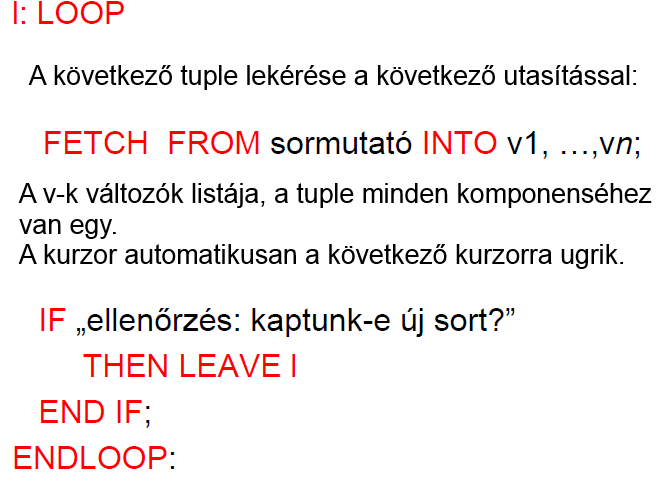
\includegraphics[width=0.45\textwidth]{img/psm3.png}
 		\caption{PSM kurzor ciklusának szerkezete}
 	\end{figure}
 	A ciklusból való kilépés trükkös pontja a kurzornak. A megoldás a következő: deklarálunk egy boolean feltételt, ami akkor igaz, ha az SQLSTATE egy meghatározott értéket vesz fel (02000, nem talált következő tuple-t).  
 	
 	
 	\subsection{PL/SQL}
	
	PL/SQL-ben nem csak tárolni lehet eljárásokat és függvényeket, hanem futtatni is lehet a ,,generic query interface"-ből (sqlplus), mint bármely SQL utasítást. A triggerek a PL/SQL része. \\
	A deklarációs rész külön válik a törzstől és opcionális, és a DECLARE kulcsszó csak egyszer szerepel a rész elején, nincs minden változó előtt. Értékadás := jellel. További különbség a PSM-hez képest, hogy paramétereknél név-mód-típus sorrendben kell megadni, és az IN OUT mód két szóban írandó. Több új típus is van, pl NUMBER lehet INT van REAL. Egy attribútum típusára lehet hivatkozni is: R.x\%TYPE. Létezik R\%ROWTYPE is,  ami egy tuple-t ad vissza. Az x tuple komponensének értékét így kapjuk meg: x.a.  ELSEIF (PSM-ben) helyett ELSIF. LEAVE ciklus helyett EXIT WHEN $<$feltétel$>$.
	\begin{figure}[H]
		\centering
		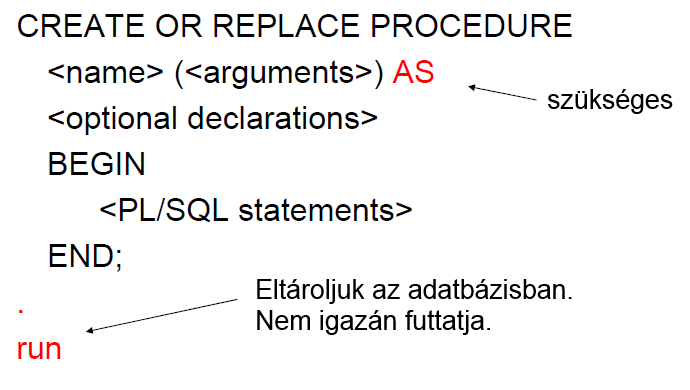
\includegraphics[width=0.45\textwidth]{img/plsql1.png}
		\caption{PL/SQL eljárás szerkezete}
	\end{figure}
	\textit{Kurzor}: CURSOR $<$név$>$ IS $<$lekérdezés$>$. A ciklusban a kurzor tuple-jének lekérése: FETCH $<$kurzor neve$>$ INTO $<$változó(k)$>$. PL/SQL-nél a kurzor ciklusát így hagyjuk el: EXIT WHEN $<$kurzornév$>$\%NOTFOUND.
	\section{Relációs adatbázis-sémák tervezése, normálformák, dekompozíciók}
	
	\subsection{Relációs adatbázis-sémák tervezése}
	
	Függőségek: funkcionális, többértékű, ezeket a tervezésnél használják (az adatbázisrendszerek nem támogatják, ott megszorítások vannak). \\
	Normalizálás: jó sémákra való felbontás, funkcionális függőségek $\to$ (1,2,)3NF, BCNF; többértékű függőségek $\to$ 4NF.
	
	\subsubsection{Funkcionális függőségek}
	
	X $\to$ Y az R relációra vonatkozó megszorítás, miszerint ha két sor megegyezik X összes attribútumán, Y attribútumain is meg kell, hogy egyezzenek. \\
	Jelölés: X, Y, Z... attribútum halmazokat; A, B, C... attribútumokat jelöl. {A,B,C} attribútumhalmaz helyett ABC-t írunk. \\
	\textit{Definíció.} Legyen R(U) egy relációséma, továbbá X és Y az U attribútumhalmaz részhalmazai. X-től \textit{funkcionálisan függ} Y (jelölésben X $\to$ Y), ha bármely R feletti T tábla esetén valahányszor két sor megegyezik X-en, akkor megegyezik Y-on is, $\forall t_1, t_2 \in T$ esetén $(t_1[X]=t_2[X] \Rightarrow t_1[Y]=t_2[Y])$. Ez lényegében azt jelenti, hogy az X-beli attribútumok értéke egyértelműen meghatározza az Y-beli attribútumok értékét. Jelölés: R $\models$ X $\to$ Y, vagyis
	R kielégíti X $\to$ Y függőséget. \\
	\textit{Jobboldalak szétvágása}: $X \to A_1A_2...A_n$ akkor és csak akkor teljesül R relációra, ha $X \to A_1$, $X \to A_2$,..., $X \to A_n$ is teljesül R-en. Példa: A$\to$BC ekvivalens A$\to$B és
	A$\to$C függőségek kettősével. Baloldalak szétvágására nincs szabály, ezért elég nézni, ha a FF-k jobboldalán egyetlen attribútum szerepel. \\
	Példa funkcionális függőségekre: Sörivók(név, cím, kedveltSörök, gyártó, kedvencSör) táblában név $\to$ cím kedvencSör (egy ua., mint név $\to$ cím és név $\to$ kedvencSör), kedveltSörök $\to$ gyártó. \\ \\
	\textit{Kulcs, szuperkulcs} Funkcionális függőség X $\to$ Y speciális esetben, ha Y = U, ez a kulcsfüggőség. R(U) relációséma esetén az U attribútumhalmaz egy K részhalmaza akkor és csak akkor szuperkulcs, ha a K $\to$ U FF teljesül. A kulcsot tehát a függőség fogalma alapján is lehet definiálni: olyan K attribútumhalmazt nevezünk kulcsnak, amelytől az összes többi attribútum függ, de K-ból bármely attribútumot elhagyva ez már nem teljesül (vagyis minimális szuperkulcs). Példa az előző alapján: $\{$név, kedveltSörök$\}$ szuperkulcs, ez a két attr. meghatározza funkcionálisan a maradék attr-kat. \\ \\
	\textit{Függőségek implikációja}: F implikálja $X \to Y$-t, ha minden olyan táblában, amelyben F összes függősége teljesül, $X \to Y$ is teljesül. Jelölés: $F \models X \to Y$, ha F implikálja $X \to Y$–et. \\
	Legyenek $X_1 \to A_1$, $X_1 \to A_2$,..., $X_1 \to A_n$ adott FF-k, szeretnénk tudni, hogy $Y \to B$ teljesül-e olyan relációkra, amire az előbbi FF-k teljesülnek. Példa: $A \to B$ és $B \to C$ teljesülése esetén $A \to C$ biztosan teljesül. $Y \to B$ teljesülésének ellenőrzésekor vegyünk két sort, amelyek megegyeznek az összes Y-beli attribútumon. Használjuk a megadott FF-ket annak igazolására, hogy az előbbi két sor más attribútumokon is meg kell, hogy egyezzen. Ha B egy ilyen attribútum, akkor $Y \to B$ teljesül. Egyébként az előbbi két sor olyan előfordulást ad majd, ami az összes előírt egyenlőséget teljesíti, viszont $Y \to B$ mégsem teljesül, azaz $Y \to B$ nem következménye a megadott FF-eknek. \\ \\
	Armstrong-axiómák: Legyen R(U) relációséma és $X,Y \subseteq U$, és jelölje XY az X és Y attribútumhalmazok egyesítését. F legyen funkcionális függőségek tetsz. halmaza. \\
	\begin{itemize}
		\item FD1 (reflexivitás): $Y \subseteq X$ esetén $X \to Y$.
		\item FD2 (bővíthetőség): $X \to Y$ és tetszőleges Z esetén $XZ \to YZ$.
		\item FD3 (tranzitivitás): $X \to Y$ és $Y \to Z$ esetén $X \to Z$.		
	\end{itemize}
	Az Armstrong-axiómarendszer helyes és teljes, azaz minden levezethető függőség implikálódik is, illetve azok a függőségek, amelyeket F implikál azok le is vezethetők F-ből. $F \vdash X \to Y \iff F \models X \to Y$\\ \\
	\textit{Levezetés}: $X \to Y$ levezethető F-ből, ha van olyan $X_1 \to Y_1$, ..., $X_k \to Y_k$,..., $X \to Y$ véges levezetés, hogy $\forall k$-ra $X_k \to Y_k \in F$ vagy $X_k \to Y_k$ az FD1, FD2, FD3 axiómák alapján kapható a levezetésben előtte szereplő függőségekből. Jelölés: $F \vdash X \to Y$, ha $X \to Y$ levezethető F-ből. \\
	További levezethető szabályok:
	\begin{itemize}
		\item Összevonhatósági szabály: $F \vdash X \to Y$ és $F \vdash X \to Z$ esetén $F \vdash X \to YZ$.
		\item Pszeudotranzitivitás: $F \vdash X \to Y$ és $F \vdash WY \to Z$ esetén $F \vdash XW \to Z$.
		\item Szétvághatósági szabály: $F \vdash X \to Y$ és $Z \subseteq Y$ esetén $F \vdash X \to Z$.
	\end{itemize}
	\textit{Attribútumhalmaz lezártja}: Adott R séma és F funkcionális függőségek halmaza mellett, $X^+$ az összes olyan A attribútum halmaza, amire X $\to$ A következik F-ből. (R,F) séma esetén legyen $X \subseteq R$. Definíció: $X^{+(F)}:=\{A | F \vdash X \to A\}$ az X attribútumhalmaz lezárása F-re nézve. Lemma: $F \vdash X \to Y \iff Y \subseteq X^+$. Következménye: az implikációs probléma megoldásához elég az $X^+$-t hatékonyan kiszámolni. \\
	Az implikációt lezárással is el lehet dönteni. Kiindulás: $Y^+ = Y$. Indukció: Olyan FF-ket keresünk, melyeknek a baloldala már benne van $Y^+$-ban. Ha $X \to A$ ilyen, A-t hozzáadjuk $Y^+$-hoz. \\\\
	\textit{FF-ek vetítése}: Motiváció: ,,normalizálás", melynek során egy reláció sémát több sémára bonthatunk szét. Példa: ABCD $F=\{AB \to C, C \to D, D \to A\}$. Bontsuk fel ABC és AD-re. Milyen FF-k teljesülnek ABC –n? Nem csak $AB \to C$, de $C \to A$ is! Vetület kiszámítása: Induljunk ki a megadott FF-ekből és keressük meg az összes nem triviális FF-t, ami a megadott FF-ekből következik. (Nem triviális = a jobboldalt nem tartalmazza a bal.) Csak azokkal az FF-kel foglalkozzunk, amelyekben a projektált séma attribútumai szerepelnek. Függőségek vetülete: Adott (R,F), és $R_i \subseteq R $ esetén: $\Pi_{R_i}(F):=\{X \to Y | F \vdash X \to Y, XY \subseteq R_i\}$.\\ \\
	\textit{A többértékű függőség} (TÉF): az R reláció fölött $X \to\to Y$ teljesül: ha bármely két sorra, amelyek megegyeznek az X minden attribútumán, az Y attribútumaihoz tartozó értékek felcserélhetőek, azaz a keletkező két új sor R-beli lesz. Más szavakkal: X minden értéke esetén az Y-hoz tartozó értékek függetlenek az R-X-Y értékeitől. Definíció: $X,Y \subseteq R, Z:=R-XY$ esetén $X \to\to Y$ többértékű függőség. A függőség akkor teljesül egy táblában, ha bizonyos mintájú sorok létezése garantálja más sorok létezését. \\
	Formális definíció: Egy R sémájú r reláció kielégíti az $X \to\to Y$ függőséget, ha $t,s \in r$ és t[X]=s[X] esetén létezik olyan $u,v \in r$, amelyre u[X]=v[X]=t[X]=s[X], u[Y]=t[Y], u[Z]=s[Z],
	v[Y]=s[Y], v[Z]=t[Z]. Állítás: Elég az u,v közül csak az egyik létezését megkövetelni.
	Példa: Sörivók(név, cím, tel, kedveltSörök) tábla. A sörivók telefonszámai függetlenek az általuk kedvelt söröktől: név$\to\to$tel és név$\to\to$kedveltSörök. Így egy-egy sörivó minden telefonszáma minden általa kedvelt sörrel kombinációban áll. Ez a jelenség független a funkcionális függőségektől. \\
	TÉF szabályok:
	\begin{itemize}
		\item Minden FF TÉF. Ha $X \to Y$ és két sor megegyezik X-en, Y-on is megegyezik, emiatt ha ezeket felcseréljük, az eredeti sorokat kapjuk vissza, azaz: $X \to\to Y$.
		\item Komplementálás : Ha $X \to\to Y$ és Z jelöli az összes többi attribútum halmazát, akkor $X \to\to Z$.
		\item Nem lehet darabolni.
		\item Állítás: $X \to\to Y$-ből nem következik, hogy $X \to\to A$, ha $A \in Y$. (A jobb oldalak nem szedhetők szét!)
		\item Nem tranzitív.
	\end{itemize}
	A veszteségmentesség, függőségőrzés definíciójában most F funkcionális függőségi halmaz helyett D függőségi halmaz többértékű függőségeket is tartalmazhat. \\
	Tétel: A $d=(R_1,R_2)$ akkor és csak akkor veszteségmentes dekompozíciója R-nek, ha $D \vdash R_1 \cap R_2 \to\to R_1-R_2$.
	
	\subsection{Normálformák}
	
	\begin{itemize}
		\item \textit{Boyce-Codd normálforma}: R reláció BCNF-ben van, ha minden X $\to$ Y nemtriviális FF-re R-ben X szuperkulcs. Nemtriviális: Y nem része X-nek. Szuperkulcs: tartalmaz kulcsot (ő maga is lehet kulcs). Ha van olyan következmény FF F-ben, ami sérti a BCNF-t, akkor egy F-beli FF is sérti. Kiszámítjuk $X^+$-t: Ha itt nem szerepel az összes attribútum, X nem szuperkulcs.
		\item Bizonyos FF halmazok esetén a felbontáskor elveszíthetünk függőségeket. \textit{3. normálformában} (3NF) úgy módosul a BCNF feltétel, hogy az előbbi esetben nem kell dekomponálnunk. Egy attribútum elsődleges attribútum (prím), ha legalább egy kulcsnak eleme. X $\to$ A megsérti 3NF-t akkor és csak akkor, ha X nem szuperkulcs és A nem prím.
		\item A \textit{4.normálforma} hasonlít a BCNF-re, azaz minden nem triviális többértékű függőség bal oldala szuperkulcs. A TÉF-ek okozta redundanciát a BCNF nem szünteti meg. A megoldás: a negyedik normálforma. A negyedik normálformában (4NF), amikor dekomponálunk, a TÉF-eket úgy kezeljük, mint az FF-eket, a kulcsok megtalálásánál azonban nem számítanak.\\
		Egy R reláció 4NF -ben van ha: minden $X \to\to Y$ nemtriviális TÉF esetén X szuperkulcs. Nemtriviális TÉF: Y nem részhalmaza X-nek, és X és Y együtt nem adják ki az összes attribútumot. A szuperkulcs definíciója ugyanaz marad, azaz csak az FF-ektől függ.
		Definíció: R 4NF-ben van D-re nézve, ha $XY \neq R$, $Y \not\subset X$, és $D \vdash X \to\to Y$ esetén $D \vdash X \to R$.\\
		Definíció: $d=\{R_1,...,R_k\}$ dekompozíció 4NF-ben van D-re nézve, ha minden $R_i$ 4NF-ben van $\Pi_{R_i}(D)$-re nézve.\\
		Állítás: Ha R 4NF-ben van, akkor BCNF-ben is van. Következmény: Nincs mindig függőségőrző és veszteségmentes 4NF dekompozíció.\\
		Veszteségmentes 4NF dekompozíciót mindig tudunk készíteni a naiv BCNF dekomponáló algoritmushoz hasonlóan. \\
		Ha R 4NF-ben van, akkor BCNF-ben is.
	\end{itemize}
	Tételek: Mindig van VM BCNF-ra és VM FŐ 3NF-ra való felbontás.
	
	\subsection{Dekompozíciók}
	
	A rosszul tervezettség anomáliákat is eredményez. A jó tervezésnél cél az anomáliák és a redundancia megszüntetése.
	\begin{figure}[H]
		\centering
		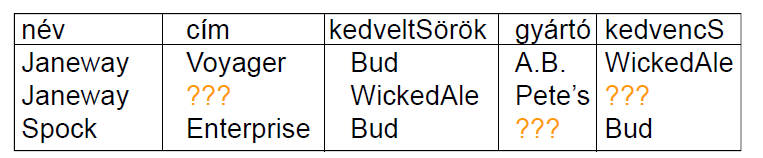
\includegraphics[width=0.6\textwidth]{img/dekomp1.png}
		\caption{Sörivó(név, cím, kedveltSörök, gyártó, kedvencSör) tábla}
	\end{figure}
	\begin{itemize}
		\item Módosítási anomália: ha Janeway-t Jane-re módosítjuk, megtesszük-e ezt minden sornál? Egy adat egy előfordulását megváltoztatjuk, más előfordulásait azonban nem.
		\item Törlési anomália: Ha senki sem szereti a Bud sört, azzal töröljük azt az infót is, hogy ki gyártotta. Törléskor olyan adatot is elveszítünk, amit nem szeretnénk.
		\item Beillesztési anomália: és felvinni ilyen gyártót? Megszorítás, trigger kell, hogy ellenőrizni tudjuk (pl. a kulcsfüggőséget).
	\end{itemize}
	\textit{Dekomponálás} (felbontás): A fenti problémáktól dekomponálással (felbontással) tudunk megszabadulni! Definíció: $d=\{R_1,...,R_k\}$ az (R,F) dekompozíciója, ha nem marad ki attribútum, azaz $R_1\cup ...\cup R_k=R$.(Az adattábla felbontását projekcióval végezzük). \\
	Elvárások:
	\begin{enumerate}
		\item Veszteségmentes legyen a felbontás, vagyis ne legyen információvesztés. A fenti jelölésekkel: ha $r = \Pi_{R_1}(r) \bowtie ... \bowtie \Pi_{R_k}(r)$ teljesül, akkor az előbbi összekapcsolásra azt mondjuk, hogy veszteségmentes. Itt r egy R sémájú relációt jelöl. Chase-teszt a veszteségmentességhez: Készítünk egy felbontást. A felbontás eleminek összekapcsolásából veszünk egy sort. Az algoritmussal bebizonyítjuk, hogy ez a sor az eredeti relációnak is sora.
		\item A vetületek legyenek jó tulajdonságúak, és a vetületi függőségi rendszere egyszerű legyen (normálformák: BCNF, 3NF def. később)
		\item Függőségek megőrzése a vetületekben (FŐ) A dekompozíciókban érvényes függőségekből következzen az eredeti sémára kirótt összes függőség. Adott (R,F) esetén $d=\{R_1,...,R_k\}$ függőségőrző dekompozíció akkor és csak akkor, ha minden F-beli függőség levezethető a vetületi függőségekből: minden $x \to Y \in F$ esetén $\Pi_{R_1}(F) \cup ... \cup \Pi_{R_k}(F) \vdash X \to Y$.
	\end{enumerate}
	A függőségőrzésből nem következik a veszteségmentesség és a veszteségmentességből nem következik a
	függőségőrzés. \\
	
\end{document}